\let\textcircled=\pgftextcircled


\chapter{Background}
\label{chap:background}

Despite recent interest in autonomous vehicles (AVs), the idea of AVs is not new. In fact, there had been attempts to autonomously navigate using cameras as early as 1990. Dan Pomerleau, a leading researcher from Carnegie Mellon, had developed a neural network, ALVINN (Autonomous Land Vehicle in Neural Network)\cite{pomerleau1989alvinn},  that could steer a van using camera input and avoid obstacles using a laser range finder . His system used artificial neural networks to categorise road and non-road segments and detect objects in them\cite{pomerleau1991rapidly}.This was one of the pioneering research in this field. Despite the success, a major limitation was the low computational power of computers at that time that led to long training times for artificial neural networks. Due to this limitation, interest in AVs slowly waned off as interest in the internet revolution peaked. 

 \begin{figure}[h]
	\centering
	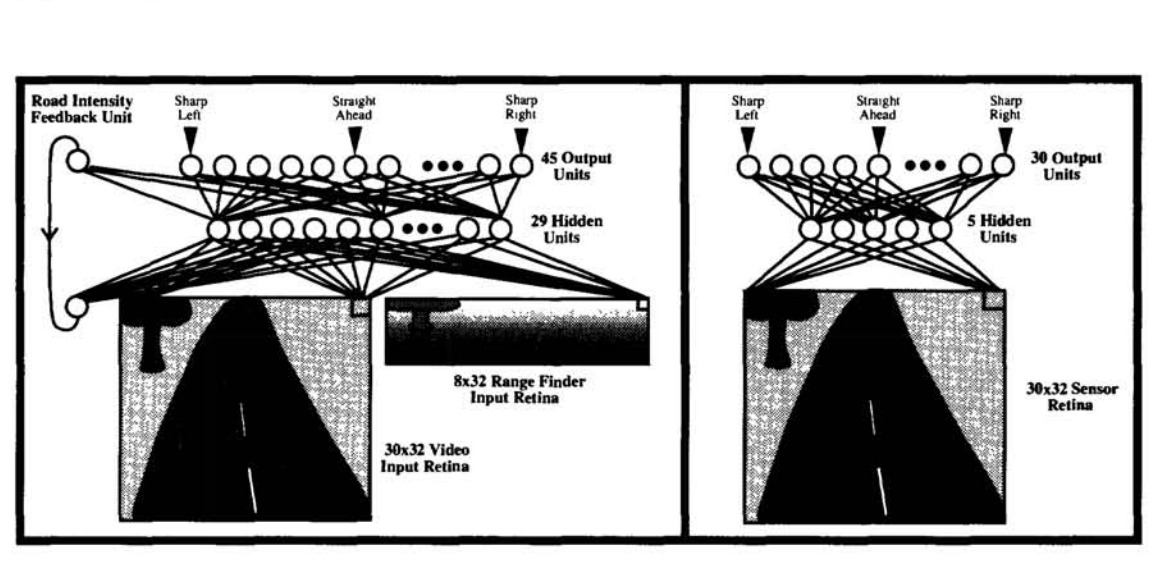
\includegraphics[width=\textwidth]{images/alvinn.png}
	\caption{ALVINN architectures. Left: With camera and laser range finder. Right: camera only. Source: \cite{pomerleau1991rapidly}}
	\label{fig:alvinn}
\end{figure}

 It was not until around 2004 when the AV landscape started seeing major development. At around this period, the US congress had passed regulation to replace 33\% of military vehicles with AVs\cite{law2001law}. Despite major military investment, there was not much progress and therefore the Defense Advanced Research Projects Agency (DARPA) opted to revolutionise the process by opening up the challenge to the public. In February 2003, DARPA hosted the Grand Challenge with a prize of 1\$ million dollars to develop an AV that could finish a 142 mile course that was set up in Mojave Desert to simulate harsh difficult conditions. Of 160 competitors, there was no winner. In the 2005 Grand Challenge, Stanford University had the fastest car to complete the course and consequently won the challenge. Subsequent challenges were held and more AVs were able to complete the course aided by advances in AI methods. Following these challenges, more research was undertaken to create more reliable and accurate sensors. Notably, Velodyne came about as a result of the Grand Challenge and is currently the leading supplier of LiDAR units. 
 
With different types of autonomous systems being deployed in vehicles nowadays, the Society of Automotive Engineers (SAE) defined five levels of autonomy to differentiate them: 
\begin{table}[H]
	\begin{tabular}{p{1cm}p{\linewidth}}
		\textbf{SAE level} & \textbf{Description}                                                                                                                                         \\ \hline
		\textbf{0}         & No AV control systems. An example is blind spot indicators.                                                                                                  \\
		\textbf{1}         & Basic driver assistance built into vehicle design. An example is the cruise control function.                                                                \\
		\textbf{2}         & Basic AV control systems. Driver required to monitor the environment and take back control if need be. A good example is the Tesla Autpilot.                 \\
		\textbf{3}         & AVs can safely navigate and drive within mapped environment. Driver required to monitor the environment and take back control if need be.                    \\
		\textbf{4}         & Highly autonomous control capable of handling most conditions but the driver has the option to take control. Renault ISymbioz is an example of a level 4 AV. \\
		\textbf{5}         & Completely autonomous with zero human intervention. None yet are available.                                 
	\end{tabular}
\end{table}


\section{Components of an AV}

\begin{itemize}
	\item \textbf{LiDAR} - LiDAR provides highly detailed 3D information about the environment around the vehicle and objects in it. LiDAR operates by sending out pulses of lasers and recording the reflections of the pulses from objects. By comparing this with the time taken for the lasers to be reflected(time of flight) and their direction, the distance of these objects can be calculated and mapped in a point cloud. 
	 \begin{figure}[h]
		\centering
		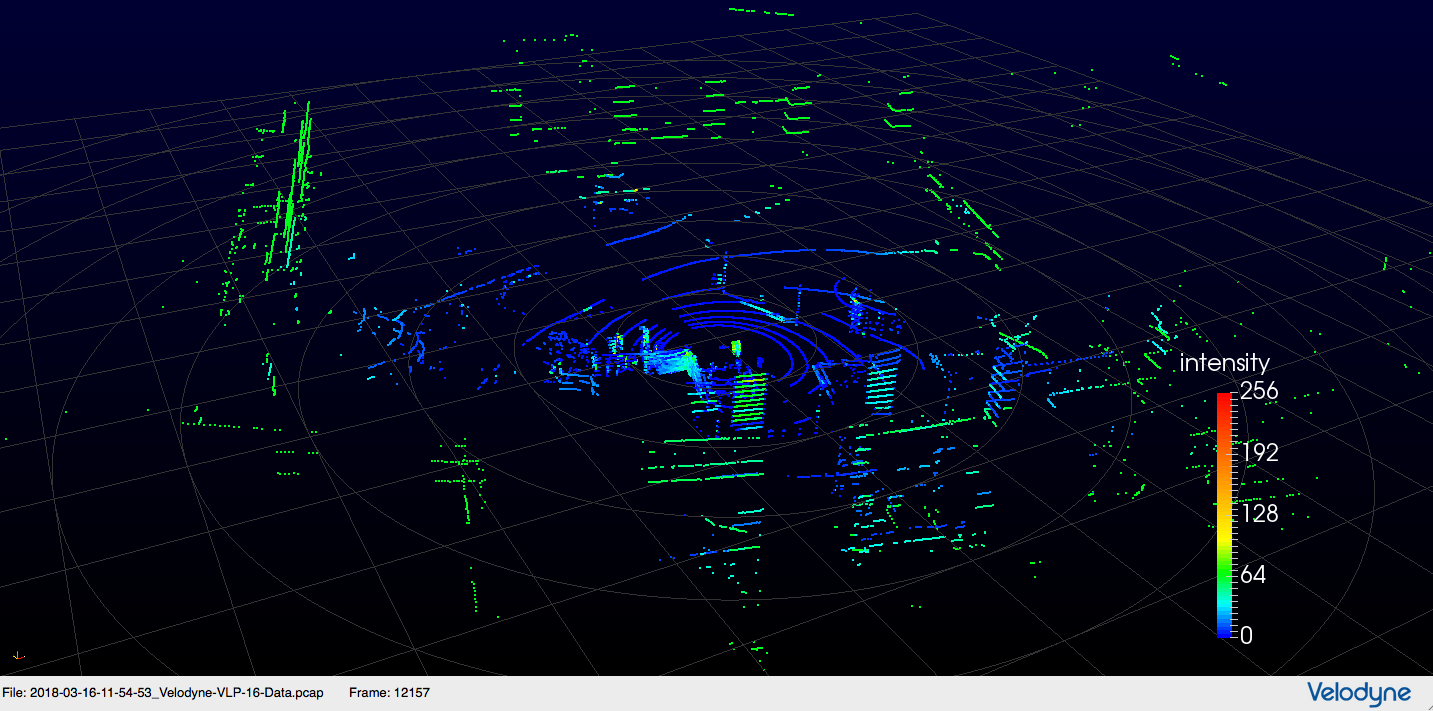
\includegraphics[width=\textwidth]{images/sil.png}
		\caption{LiDAR Point Cloud}
		\label{fig:lidar}
	\end{figure}
	LiDARs have proven to be extremely important for safe navigation due to their high level of accuracy. However due to their low angle resolution they are not able to capture contours of objects. In addition they do not provide texture information and therefore classifying objects can be quite difficult. 
%	LiDAR units require complex optical systems that are expensive to build. As a result,  they are the most expensive sensors in AVs with the top end such as Velodyne HDL-64E shown in figure \ref{fig:lidar} costing more than 50,000\$. 
%	In a bid to reduce the cost of LiDAR units,  different companies are exploring different design methods that are cheaper but still able to offer the same performance as the top end LiDAR units such as solid state LiDAR.
	
	 \begin{figure}[h]
	 	\centering
	 	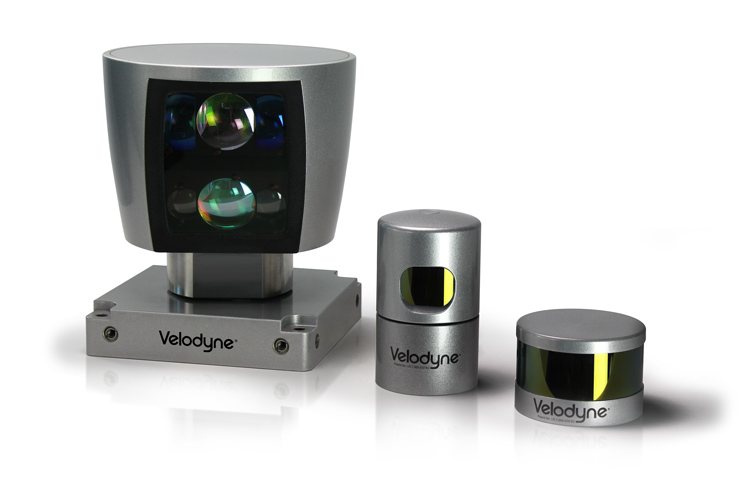
\includegraphics[width=\textwidth]{media/hdl-family.png}
	 	\caption{Velodyne LiDAR family. From left: Velodyne HDL-64E , HDL-32E , VLP-16. Source: Velodyne} 
	 	\label{fig:lidar}
	 \end{figure}
	
	\item \textbf{Cameras} -
	Grayscale and color cameras are normally used to detect and classify different objects, markings and signs on the road. Grayscale images tend to offer better edge information than color images. This can be useful for better edge detection. 
	Point clouds can also be obtained by using two cameras to obtain a stereo image that has depth information or by combining a camera and infrared laser to obtain RGB-D images such as in the Kinect sensor. 
	Less commonly, thermal cameras have been used in AVs to overcome weaknesses of color and grayscale cameras in poor lighting conditions.
	
	\item \textbf{Position Estimators} - Position estimators are a group of sensors used for navigation of the vehicle. These include GPS systems, odometers and gryometers. 
	\item \textbf{Distance Sensors} - Distance sensors such as radars and sonars are important for gauging the distance of objects on the road. 
	Radars are the most commonly used distance sensors and they function by transmitting radio waves and recording the reflected radio waves from objects. As compared to cameras and LiDARs, radars work well in a variety of low visibility scenarios such as in heavy snow/rainfall. However, the reflectivity of these radio waves depends on the nature of objects, their size, absorption characteristics and the transmitting power. As such, it is may not be effective for detecting objects with low absorption characteristics such as pedestrians and animals.
	
	\item \textbf{Processing Unit} - In order to process all the data in real-time from sensors on the vehicle, AVs require powerful processing units. Most ML/AI algorithms used for detecting and identifying objects from LiDAR and camera data demand large amounts of processing power. This is achieved through the use of CPUs, GPUs, Field Programmable Gate Arrays (FPGA)\cite{brown2012field}, Application Specific Integrated Circuits (ASICs)\cite{smith1997application} or combinations with each other. 

\end{itemize}




These components are used in different operations. In most AV implementations, these operations can be grouped into three categories:

\begin{wrapfigure}{r}{0.5\textwidth}
	\centering
	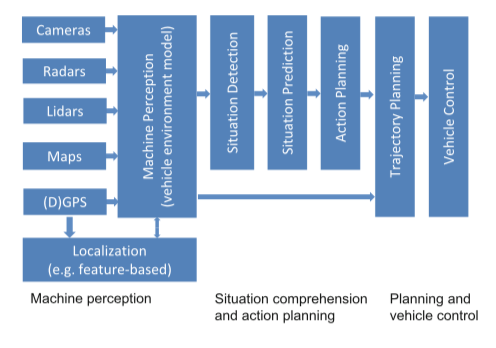
\includegraphics[width=0.48\textwidth]{images/operations}
	\caption{Detailed operation pipeline. Source:\cite{dietmayer2016predicting}}
\end{wrapfigure}

\paragraph{Perception}This is the first step which involves processing the input from the sensors. In this mode tasks such as object detection and tracking, lane detection, traffic sign detection and recognition are performed.
\paragraph{Planning}This is the next step after detection and recognition tasks are performed . In this stage route and trajectory planning algorithms are run to plan how the vehicle should navigate in the immediate environment as well as a route to a target location. These algorithms are required to handle complex situations to ensure safety of the passengers and other road users. 
\paragraph{Control}This stage involves the execution of plans created in the planning stage. This stage is crucial as the actuators involved in steering and movement have to be able to accurately follow the planned routes and actions. At this stage the trajectories and movement of other road users and objects have to be calculated in order to anticipate and avoid any accidents. 
	

\section{Industrial Approaches}
Despite improvements in traffic safety over the years, over  2.2$\%$ of deaths globally are caused by road accidents. Of these accidents, 94$\%$ are as a result of human error. A major motivation for the development of AVs is their potential to drastically reduce this by removing the human element. However due to the multidisciplinary nature of AVs there are various factors that need to be considered before public adoption of AV


\subsection{Legal and Economic Concerns}
\subsubsection*{Modelling Risk}
\begin{wrapfigure}{r}{0.5\textwidth}
	\centering
	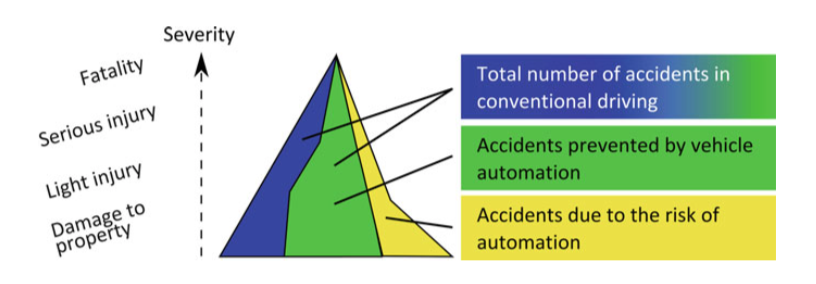
\includegraphics[width=0.48\textwidth]{images/risk}
	\caption{Diagram illustrating distribution between types of risk and severity. Source:\cite{gasser2016fundamental}}
	\label{fig:riskrel}
\end{wrapfigure}
Gasser et. al\cite{gasser2016fundamental}, define safety as the lack of unreasonable risks where risk is the product of the probability of an accident and its severity. From this, it is clear that there are different degrees of severity each with a various weighting; a fatality is more costly than damage to property. In their study they were able to establish that AVs will have the potential of preventing some accidents, however, they will introduce some risk as a result of their automation. They further went on to establish the relationship with severity as seen in figure \ref{fig:riskrel}. From this relationship they speculated that there is no uniform distribution of risk and in addition, there may be a reduction in severe accidents but an increase in lesser severe accidents. 
This relationship can be expressed as a ratio that could express the probability of  acceptance of a said autonomous system. 
\begin{equation*}
P_{acceptance} = \frac{R_{added\, risk}}{R_{avoided\, risk}}
\end{equation*}

However, this ratio does not necessarily guarantee approval as there are some cases of certain systems such as nuclear plants that the risks outweigh the benefits but due to socio-economic and/or political factors tend to get accepted. Nonetheless, it forms a pragmatic ratio that could be used as a rule of thumb.
\subsubsection*{Liability}
In terms of safety, a lot of arguments against fully autonomous vehicles have been based on trolley problems whereby the AV has to choose between two fatal scenarios, either killing the passenger or by standers in the case of an accident. However this argument has quite a few vital flaws as outlined in \cite{fried2012does}. It was established that most tragic choices are avoidable by undertaking enough preventive measures. This has been the basis for most AV systems whereby they practise minimal risk policy.  Waymo define an "operational design domain" whereby their AVs can safely operate. This includes time of day, speed ranges, traffic laws and regulations among other factors\cite{waymo_2018}. This ensures that the vehicle is able to maintain minimal risk operation. Coupled with the sensors continually monitoring vehicles and objects around them, they are able to continuously preempt potentially dangerous situations and avoid them. In addition, backup systems are installed to increase the level of redundancy in case some systems fail.

As mentioned before, there is a risk associated with the introduction of these AVs that may result in accidents. As a result, shifting from human agents to an autonomous agent will result in creation of a large number of legal questions in terms of liability and safety regulations. Currently there is no legal framework that cover the use of fully autonomous vehicles. 
 Manufacturers developing AVs will need to develop robust and reliable systems to a satisfactory degree so as not to open themselves to product liability suits. A leading cause of product liability suits is accidents when using their automotative products. In addition, this can further extend to the use of a defective design on the vehicle even when there is no accident by the concept of strict liability. Another consideration that can lead to litigation is the breach of warranty. According to \cite{wu2015product}, a warranty is "an affirmation or promise concerning a product or its performance, features, or characteristics, such as those concerning the safety of a product". 
In light of this, companies developing AVs need to consider the following as defined in \cite{wu2015product}:
\begin{itemize}[noitemsep]
	\item Design systems  that are highly accurate and able to recognize other road users and hazards.
	\item The systems should be able to use enough data from sensors at real-time and process to a high precision. 
	\item Develop sufficient crash avoidance strategies. 
	\item Ensure adequate information security measures are undertaken.
\end{itemize}
Nonetheless, it is also important to create a collective scientific examination process that investigates how the traffic system that is used currently may contribute to accidents \cite{gasser2016fundamental}. This has  been the basis for developing traffic systems to be used in case of 100\%  AV adoptions such as \cite{tachet2016revisiting}. 


\subsection{Hardware Considerations}
In light of the legal requirements,  \cite{lin2018architectural} established a few metrics that could be used in order to achieve viable AV systems.
		
\subsubsection*{Performance} 
At the moment there are no clear regulations as to how fast the perception, planning and control pipeline should be. However according to research by Brown et al. \cite{brown1994human}, humans take around 600 ms to respond and brake when expecting an interruption, however this figure shoots to 850 ms when an unexpected situation arises. In addition, Newell et al \cite{newell1985prospects}, established that the fastest human response time is between 100-150ms. These figures can be used as a baseline while developing a pipeline. In this pipeline, there are two factors to consider, namely the frame rate (frequency of the data from sensors) and the processing latency (time taken to process data). In consideration of this, \cite{lin2018architectural} estimated that an AV system should be able to run processed within 100ms to achieve better performance than a human driver. 

\subsubsection*{Storage} 
AVs should be able to store maps of different areas with fine granularity for accuracy during localisation. As a result, the storage of these maps can run into tens of Terabytes. Despite recent advances in cloud technology and the emergence of 5G connectivity that is significantly fast. Downloading these maps would take significant time and would also render the car unusable in case of no internet connectivity. As such, the vehicles should have enough storage to store these maps locally. 

\subsubsection{Power} 
\begin{wrapfigure}{R}{0.5\textwidth}
	\centering
	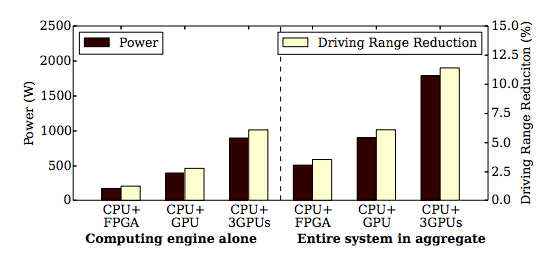
\includegraphics[width=0.48\textwidth]{images/power_reduction}
	\caption{Graph illustrating reduction of power range against the processing unit configurations. Source:\cite{lin2018architectural}}
	\label{fig:powerred}
\end{wrapfigure}
Most of the major industry players have moved to electric-vehicles for their AV systems. Depending on the equipment and sensor configurations used in these systems, the power usage can range from 500 watts to 1.5 kilowatts. Total power consumption includes the computing, storage and cooling overheads. Given that the AVs have limited battery capacity, heavy power consumption by these systems can lead to poor driving ranges hence making the cars less viable.
From their evaluation, a system with 1 CPUs and 3 GPUs operating fully can lead to a 6\% reduction in the driving range and 11.5\% if the whole system is considered. Furthermore, they established that cooling such a system would result in a 77\% overhead of the total power usage.
Therefore,  the configuration of these systems has to be carefully considered to ensure a reasonable driving range. 

\subsubsection*{Thermal} 
Processing components in the AV systems such as CPUs and GPUs require a significant amount of energy to cool. This is necessary to ensure that they operate within their recommended thermal operating range. Failure to do so could result in the failure of these systems.  Depending on the type of component, the range is normally below 80\degree Celcius. Additional cooling systems are therefore necessary to ensure optimal operating temperatures. 

\subsection{Perception}
Following the discussion above, the next subsections will review how different industry players are implementing their AV systems with special focus to the issue of perception. Figure \ref{fig:players} illustrates the current progress of various companies working on AVs.
\begin{figure}
	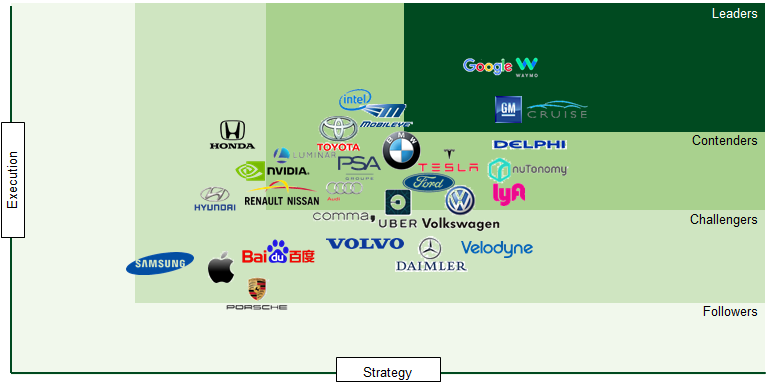
\includegraphics[width=\textwidth]{media/avind.png}
	\caption{AV Leaderboard by Navigant Research. Source:\cite{navigantresearch_2018}}
	\label{fig:players}
\end{figure}
\subsubsection*{Camera Only}
Mobileye\cite{mobileye_2018}, is one of the top contenders in the development of camera only AVs. They were recently acquired by Intel and believe that AVs should be able to accurately and safely navigate using cameras only given the fact that humans are able to do so with vision only. Previously, MobilEye was a supplier of vision systems for Advanced Driver Assistance Systems and had a partnership with Tesla to supply their vision systems prior being acquired by Intel. 
Given their extensive background in developing these vision systems, the partnership with Intel aims to develop a complete autonomous driving package\cite{intelsolutions_2018}.
 

\subsubsection*{Camera and  Radar}
Another major contender that is using the camera and radar configuration is Tesla. Elon Musk, the founder, believes that LiDAR is not necessary for AV perception following a similar argument as MobilEye. However, this argument was dispelled following a recent crash whereby due to bright sunlight, a Tesla vehicle on 'autopilot' mode was unable to detect a white vehicle thus resulting in an accident leading to loss of life. The invariance of LiDAR to different lighting conditions could have helped in detecting the vehicle. 

\subsubsection*{LiDAR, Camera and Radar}
This configuration is used by most of the leading industry players such as Uber, Waymo and GM Cruise. This configuration has proven to be robust and accurate. However, in order to process the amount of fused data, they require large amounts of computational power which in turn may lead to increased power usage. 
\begin{figure}[t]
	\centering
	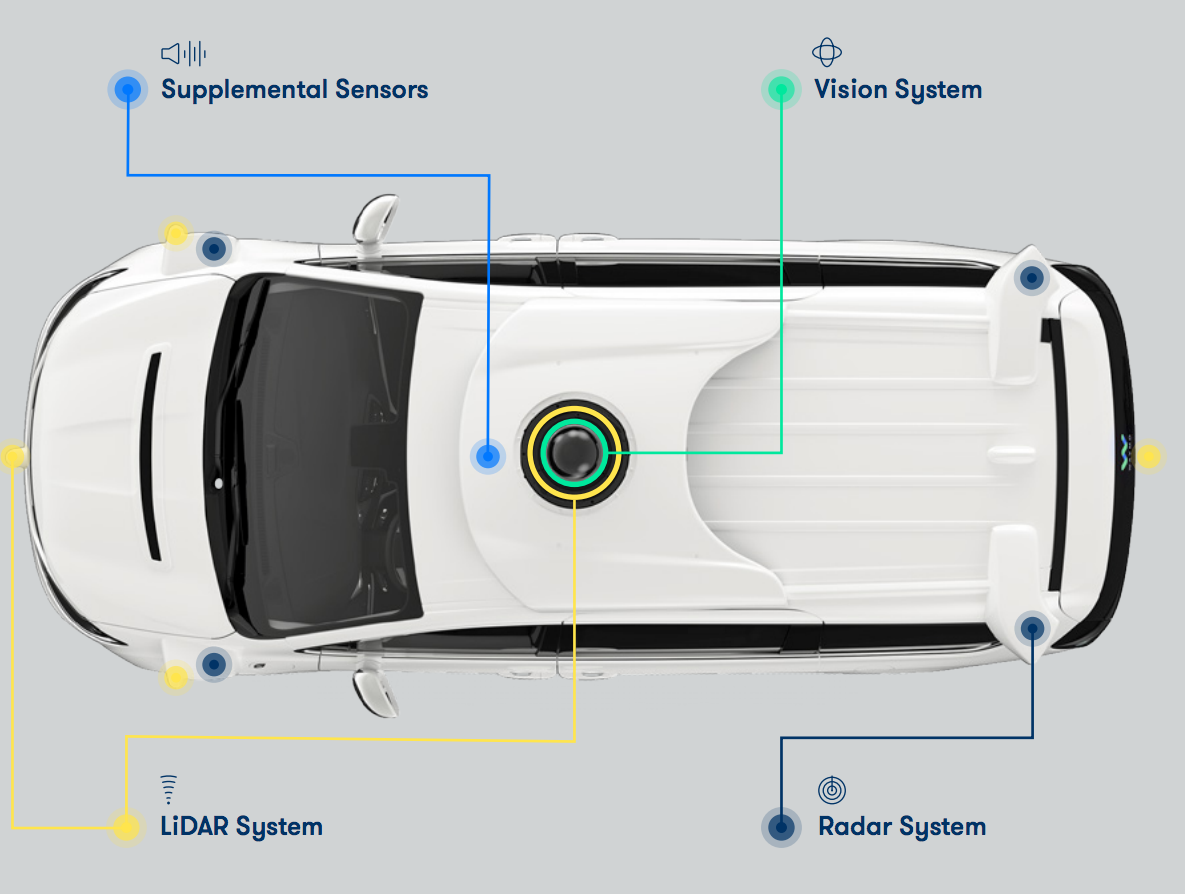
\includegraphics[width=\textwidth]{media/waymo.png}
	\caption{Waymo's Self Driving Car Configuration, Source:\cite{waymo_2018}}
	\label{fig:waymo}
\end{figure}
\subsubsection*{LiDAR }
LiDAR-only systems have not been explored by major companies working on AVs for driving on public roads. However,various autonomous robots have been developed to assist in other industries such as the Neato house cleaning robot. Doxel, a start up aiming to solve problems in the construction industry has also created an autonomous robot that autonomously scans and captures the progress of different construction sites and further process them using neural networks.
\section{Object  Detection} 
Object detection has seen a rapid increase in innovation over the past few years. From the early days of the sliding window method used in classic computer vision algorithms to the development of deep learning algorithms that are able to learn complex features automatically. 
In this section, I will explore different object detection methods that have been used and their underlying methods of operation.

\subsection{Object Detection using Classic Computer Vision Methods}
Classic computer vision methods have advanced over the years from simple algorithms such as SIFT\cite{lowe1999object} and SURF\cite{bay2006surf} which use descriptors to detect interesting points in images for object detection to much higher level representations such as the Histogram of Gradient (HOG)\cite{dalal2005histograms} or Haar Features\cite{viola2001rapid}  that were used in classifiers applied on a sliding window. 

However, these methods have been unreliably slow and not as accurate. In addition these features are only able to model 2D data. 3D methods such as Intrinsic Shape Signatures(ISS)\cite{zhong2009intrinsic}, NARF\cite{steder2010narf} and Uniform Sampling have since been developed but are lacking in terms of speed. Furthermore, these feature detectors have to be hand-crafted manually which is a tedious process. As a result, they are rarely used in real-time AV applications due to their speed and accuracy.

\subsection{Object Detection using Deep Learning}
The advancement of neural networks has offset the reliance of classical methods of object detection by allowing for features to be automatically learnt by the network without the need for manual feature extraction. This is attributed to the networks having a numerous number of deep layers that are able to capture these features.  
\subsubsection*{Convolutional Neural Networks (CNN)}
CNNs have been there for over two decades now and are inspired by the idea of receptive fields in the primary visual cortex. Currently, they are widely used in image object detection tasks and various CNN architectures have been developed. As compared to regular neural networks which have all neurons connected to each other between hidden layers, neurons in CNNs are connected to a small region in the layer before it(receptive field) and have three dimensions(width,height and depth). By doing so this reduces the number of parameters to be tuned during back-propagation as well as to be stored. 
\begin{figure}[h]
	\centering 
	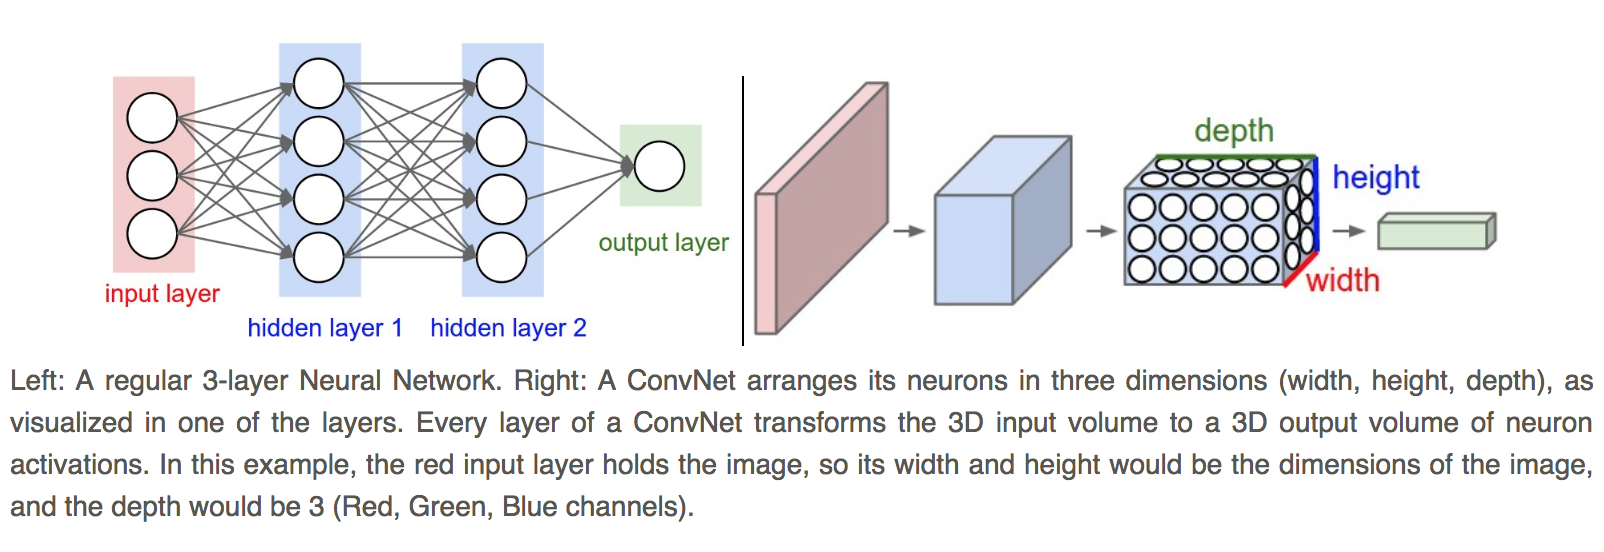
\includegraphics[width=\linewidth]{images/neuralnet}
	\caption{NN vs CNN Source: \url{https://cs231n.github.io/convolutional-networks}}
	\label{fig:cnn}
\end{figure}


Common architectures implement five main layers. 
\begin{itemize}[noitemsep]
	\item  \textbf{Input Layer} Forms the first stage of the CNN where the input data is fed in.
	\item  \textbf{Convolution Layer} This layer calculates the output of neurons connected to a receptive field.
	The size of the output is determined by the following equation. 
	
	$A_{out}= (A_{in}-K+2P)/S+1$
	
	where $A_{in}$ is the input size,  $A_{out}$ is the output size, K is the kernel size, P is the padding size and S is the stride of the kernel. 
	\item  \textbf{Activation Layer} In this layer the output of the convolution is passed through an activation function such as sigmoid, ReLU or TanH. 
	\item  \textbf{Pooling Layer} This layer downsamples the  output of the activation layer along the width and height dimensions. 
	\item \textbf{Fully connected layer} Finally, this layer computes the probability scores for different classes by connecting all neurons from the pooling layer. 
\end{itemize}

\subsubsection*{Region Proposal Networks(RPN)}
R-CNN\cite{girshick2014rich} brought forth the idea of region-based CNNs with the aim of increasing the accuracy of CNNs. By using selective search, regions of interest(ROI) in input images are proposed. These regions are then resized and fed through a CNN to generate a bounding box and classification of the image. Finally a classifier and regressor are run on the output. However, as this method requires a forward pass of the CNN for each proposal, its speed was quite slow. In addition, the CNN, classifier and regressor have to be trained and tuned separately. 
Fast R-CNN\cite{girshickICCV15fastrcnn} iterated on R-CNN to further improve the speed and accuracy by using ROIPooling whereby instead of running each proposal in a CNN, regions that were overlapping were pooled and fed through the CNN thus sharing the computation. Furthermore, this model was end-to-end and thus combined the classifier and regressor  by adding a softmax layer and linear regression layer after the CNN.
Faster R-CNN\cite{ren2015faster} sought to remove the bottleneck imposed by the using selective search to propose regions. This was solved by using a sliding window with various anchor boxes on feature maps generated by a forward pass of a CNN. Bounding boxes on certain regions of the image could be generated. These regions are then passed onto Fast R-CNN to classify the objects. 
\begin{figure}[h]
	\centering
	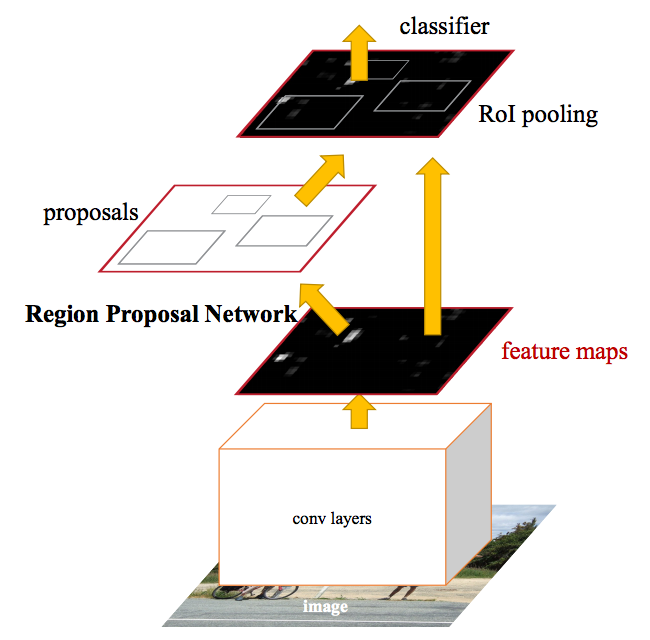
\includegraphics[width=0.5\linewidth]{images/fastercnn}
	\caption{Faster R-CNN overview. Source:\cite{ren2015faster}}
\end{figure}


Depending on the input, these two network architectures have formed the back bone of most 2D and 3D object detection applications. 
\paragraph{Monocular Vision} 
Monocular vision is derived from a single camera. This representation is 2D and lacks depth information. Mono3D\cite{chen2016monocular} by Chen et al.  is a state of the art object detection model that uses monocular images where they were fed through a CNN and the resulting 2D object proposals were extruded into 3D bounding boxes by performing segmentation.

\paragraph{Stereo Vision}Stereo vision involves calibrating two cameras intrinsically and extrinsically by matching similar points in images from both cameras. Using the resulting stereo image, it is possible to estimate the depth of objects in the image. However the accuracy of this depends on a few factors such as the resolution, camera quality, lens distortion and the calibration algorithm. 3DOP \cite{chen20183d} is one of the state-of-the-art models that uses stereo images in CNNs to detect objects.  

\paragraph{LiDAR+Camera}
By fusing input from a monocular image and point clouds, it is possible to extract depth information from the images. Chen et al further reiterated their monocular approach into MV3D\cite{chen2017multi} a multiview 3D object detection network. In their work, they were able to fuse LiDAR and camera input to create a bird's eye view of the surrounding environment and further perform object detection of features. 


\paragraph{LiDAR} 
Point cloud object detection is particularly challenging as established 3D object detection methods for images cannot be applied to point clouds. Point clouds are a set of geometric points in a euclidean space. They are unordered in nature and this presents a particular problem to deep learning methods as they need to be invariant to permutations of the input set.
Depending on how they manipulate the point clouds, current point cloud based object detection models can be split into three groups:
\begin{enumerate}
	\item \textbf{Direct Manipulation} \\ 
	Pointnet\cite{qi2017pointnet} developed by Qi et al was able to overcome this challenge on small sets of point clouds. By using point clouds as direct input into Recurrent Neural Networks\cite{medsker2001recurrent} They were able to create a global point cloud signature that could classify and segment 3D objects in the point cloud. They further improved this model into Pointnet++\cite{qi2017pointnet++} which recursively applied PointNet on nested partitions of the point clouds using a hierarchical neural network. In doing so they were able to capture the local structures of the point clouds as a result of their metric nature and thus achieve better performance than PointNet. However this approach has high memory and computational requirements. For both of these publications, the source code was released for public use. Consequently, they have formed a fundamental foundation for further development of point cloud object detection methods such as F-PointNet\cite{qi2017frustum}.
	
	\item \textbf{Voxel Based} \\
	By dividing the pointclouds into 3D voxel grids, points within these voxels can be sampled to perform feature extraction. VoxelNet \cite{zhou2017voxelnet} is a state of the art architecture that uses this method to extract these features through Voxel Feature Extraction layer. The extracted features are then fed through a RPN to generate bounding boxes and classify objects within them. 
	
	\item \textbf{2D-Based }\\
	This involves projecting the pointcloud into a 2D image plane coordinate system which can then be trained on existing image based CNNs  such as VGG-16. VeloFCN \cite{li2016vehicle} was one of the first methods to implement this approach using a fully convolutional network. However, VeloFCN lacked bird eye and front view representations. 
	
\end{enumerate}



\begin{table}[h]
	\centering
	\begin{tabular}{|l|l|l|l|}
		\hline
		\textbf{Network Model} & \textbf{Mode}         & \textbf{Code} & \textbf{Inference Time}  \\ \hline
		\textbf{VoxelNet}      & \textit{LiDAR}        & Unnoficial    & \textit{\textbf{100ms}} \\ \hline
		\textbf{AVOD}          & \textit{LiDAR+Image}  & Yes           & \textit{\textbf{100ms}} \\ \hline
		\textbf{MV3D}          & \textit{LiDAR+Image}  & Unnoficial    & 360ms                   \\ \hline
		\textbf{MONO3D}        & \textit{Mono Image}   & Yes           & 4.2s                    \\ \hline
		\textbf{3DOP}          & \textit{Stereo Image} & Yes           & 3s                      \\ \hline
	\end{tabular}
	\caption{Modes of Operation of Common Architectures}
	\label{tab:arch}
\end{table}






%A major topic of concern that has been raised consistently in the development of AVs is the safety of these systems especially 
%Despite improvements in traffic safety over the years, over  2.2$\%$ of deaths globally are caused by road accidents. Of these accidents, 94$\%$ are as a result of human error. It has been argued that AVs will reduce this figure by 
%
%According to \cite{gasser2016fundamental}, there are no public laws that cover the  use of independent autonomous vehicles in public spaces. In his article, he cites the fundamental issue as "understanding and accepting the effect of AVs as an independent action by a machine". Due to the lack of public laws on their use, he proposes extending fundamental rights such as the right to life into the framework for creating laws that cover emerging technologies that have an effect on the public, that are otherwise not accounted for in traditional laws.
%
% 
%Bearing this in mind, it is important to note that  It has been predicted that upon mainstream 
%
%This creates a realistic baseline that can then be extended in evaluating the performance of AV systems. As such, if the risk of automation is lesser than the risk of human vehicle control then the AV would be beneficial. Consequently, the AVs are not to be considered as perfect systems but instead should be treated as systems that minimise the overall risk to the passenger and also their surroundings. 



%
%
%
%The classic ethical dilemma for self driving cars poses a scenario whereby AVs are presented with a situation whereby a fatal accident is inevitable. For example, the AV either has to crash into a group of people in order to save the life of a passenger or to crash itself and sacrifice the life of the passenger. This dilemma highlights important legal, ethical and economic considerations to be considered by companies involved in the production of AVs and their corresponding systems. 
%
%
%According to \cite{gasser2016fundamental}, there are no public laws that cover the  use of independent autonomous vehicles in public spaces. In his article, he cites the fundamental issue as "understanding and accepting the effect of AVs as an independent action by a machine". Due to the lack of public laws on their use, he proposes extending fundamental rights such as the right to life into the framework for creating laws that cover emerging technologies that have an effect on the public, that are otherwise not accounted for in traditional laws. 
%
%Bearing this in mind, it is important to note that despite improvements in traffic safety over the years, 94\% are still caused by human beings with a large majority of them being fatal with the current human error rate being 1 in 100 million miles. This creates a realistic baseline that can then be extended in evaluating the performance of AV systems. As such, if the risk of automation is lesser than the risk of human vehicle control then the AV would be beneficial. Consequently, the AVs are not to be considered as perfect systems.
%
%With regard to economic considerations, car manufacturers involved in the production of AVs have to ensure that their AVs are able to handle numerous scenarios even if they are rare or considered statistically impossible. They should also be required to take legal liability in case any of their system components are defective and result in failures or accidents. This is important for customer trust without which they will not be able to convince customers to shift to AVs. In addition, for the adoption of AVs to be widespread, they have to be reasonably priced and efficient. With the current prices of the the various components and their power consumption, the adoption of AVs at the moment is not viable. 
%
%\section{Conclusion} 
%
%This chapter was opened with a brief history and motivation for AVs and the different components that are used in their development. Following this, 
% 
% An interesting point that has been established is the use of LiDAR only methods for use in AVs. 
% 
% 
%
%In addition a discussion on current approaches that are being explored 
%where we were able to 
%
%Shift from classic computer vision to deep learning methods. Where 
%Finally a discussion on 
%
%From these discussions, I came up with the following hypothesis. 